 The proposed biomechanical model consists of two bodies, one representing the pectoral cage with the pectoral muscle,	  and the second representing the breast soft tissue. Between the two bodies, a contact surface is defined in order to model tissues mechanics at the juncture interface.
 
The next section describes the implementation of different interaction models tested during the model development process. Since the breast tissues are always attached to the pectoral muscle (Figure \ref{fig:contactsurface}), the contact surface was modeled using \textit{bonded} and \textit{no-separation frictional} interaction model only.

\begin{figure}[!h]
\centering
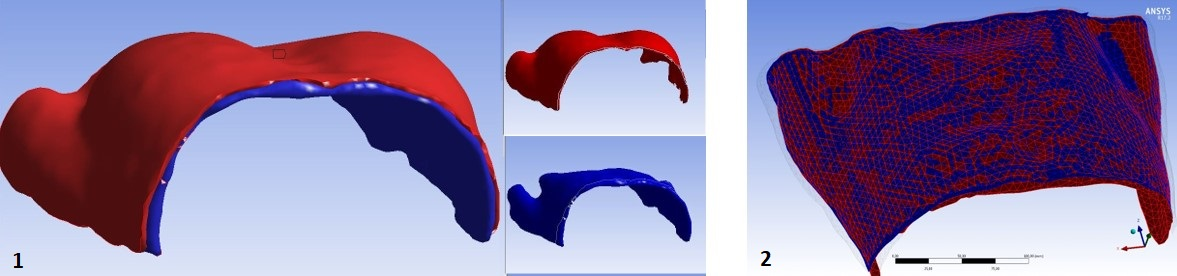
\includegraphics[width=0.9\textwidth,keepaspectratio]{figures/contactSurface.jpg} 
\caption{The two bodies representing the thoracic cage and breast (1) with their the associated contact surface (2).  Blue surface - muscle representing the target surface, red surface - breast representing contact surface}
\label{fig:contactsurface}
\end{figure}

The results for pure bonded and pure no-separation sliding models, as well as one combined contact surface, are listed bellow. For some contact models, because of large instabilities or a poor fidelity to the real breast mechanics, only partial results are presented.  

\subsubsection*{Bonded contact surface}

First, a pure bounded contact was used to model the interaction between the breast and the pectoral muscle. To achieve realistic breast deformation, extremely low values of equivalent Young's modulus and Poisson ratio were needed ($\lambda_{breast} = 0.3kPa$ and $\nu_{breast} = 0.45$).  
An example of breast deformation in prone and supine configuration is illustrated in Figure \ref{fig:bondedcontact}.

\begin{figure}[!h]
\centering
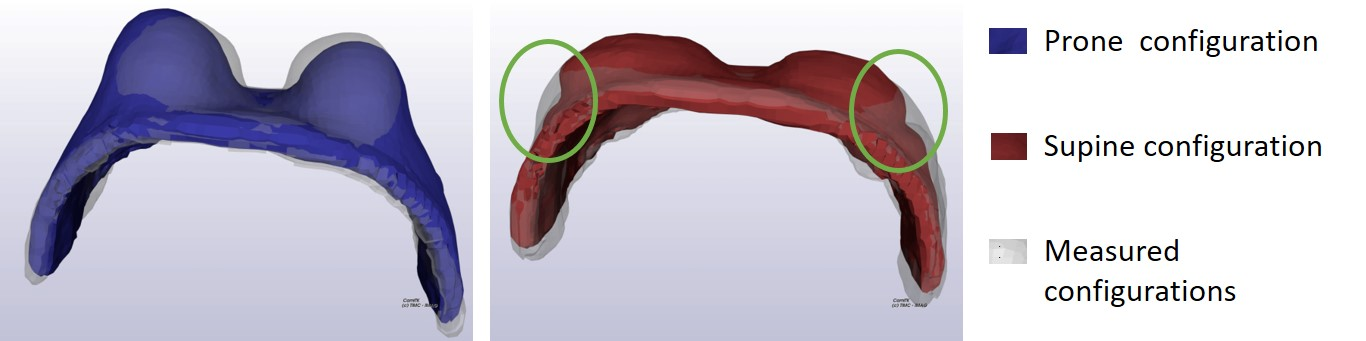
\includegraphics[width=0.9\textwidth,keepaspectratio]{figures/bondedcontact.jpg} 
\caption{Resulting breast deformation with a bonded contact model.}
\label{fig:bondedcontact}
\end{figure}

One can see that, even if the breast geometry in prone position is well estimated, the ones in supine and supine tilted configurations are constrained laterally. Moreover, an important volume variation was observed which is not a characteristic of breast changes under gravity loading. The volume variation is due to a too low value of the Poisson ratio. 

\subsubsection*{Sliding contact surface}

Pure sliding contact surface was considered in order to allow larger tissues displacements on lateral direction. The breast sliding over the muscle surface was modeled using the Coulomb friction low (Section \ref{subsection:surfaceinteractionmodels}). Additional boundary conditions were set by imposing zero-displacement on the right, left, superior and inferior mesh boundaries representing the breast volume (see Figure \ref{fig:meshboundaries} for a recall on different mesh boundaries).  This model caused large convergence problems because of breast tissues over-sliding. It was obvious that the model needs more boundary conditions in order to achieve convergence. Moreover, a non-linear and a non-uniform sliding model was needed in order imitate the behavior of rich fibrous areas where the breast is attached to the chest wall (see Section \ref{subsection:internalstructures} for a recall on breast anatomy). 


\subsubsection*{Mixt contact surface}

In order to limit breast tissues sliding, a mixt contact surface was defined. Herein, the contact surface consists of two complementary areas (Figure \ref{fig:mixtcontact}), the first one modeled as bonded contact and the second one modeled as no-separation sliding contact. The regions corresponding to the bounded contact are defined following the anatomical structures where the concentration of fibrous tissues is significantly higher. Such regions are encountered along the muscle surface where the superficial muscle fascia meets the breast suspensory ligaments, as it is the case for the inframammary ligament, the deep medial ligament or the deep lateral ligament.

\begin{figure}[!h]
\centering
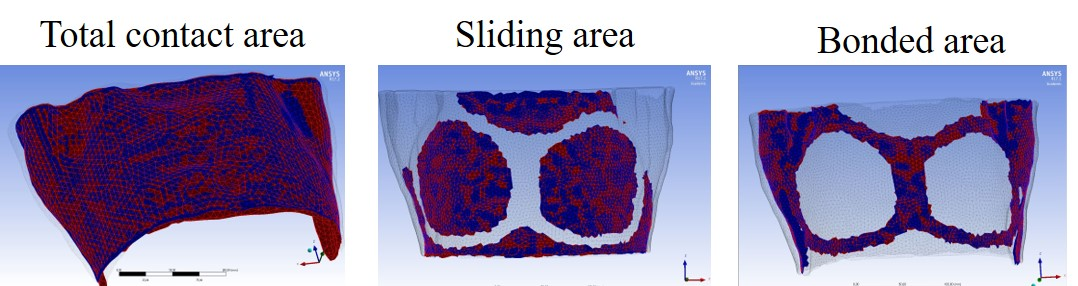
\includegraphics[width=0.9\textwidth,keepaspectratio]{figures/mixtcontactarea.jpg} 
\caption{The contact surface divided in two regions: sliding region and bonded region.}
\label{fig:mixtcontact}
\end{figure}

Using such a contact model improves substantially the estimate of the supine breast configuration. However, because of a high deformation gradient imposed at the juncture border between the two contact areas, convergence problems were observed. Moreover, when the supine configuration is estimated, several folds are created at the skin surface (Figure \ref{fig:mistcontactresults}). The same types of folds were obtained in supine tilted configuration creating large convergence problems because of tissues superposition.

\begin{figure}[!h]
\centering
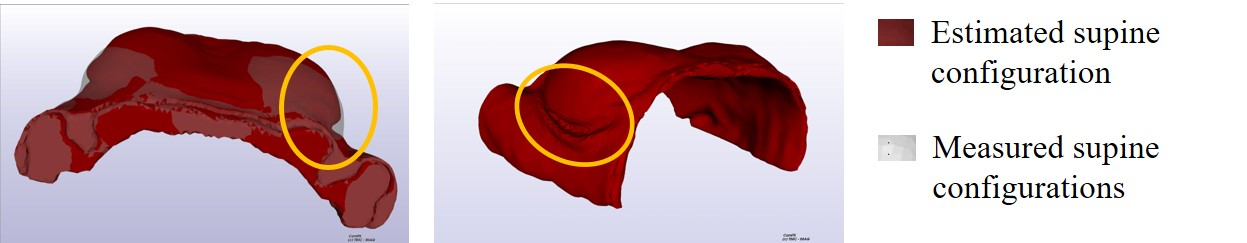
\includegraphics[width=0.9\textwidth,keepaspectratio]{figures/mixt_contact_supine.jpg} 
\caption{The contact surface divided in two regions: sliding region and bonded region.}
\label{fig:mistcontactresults}
\end{figure}

This last described model has provided satisfactory results, however it led to important solution convergence problems. Therefore, the model was improved by replacing the bonded contact regions with stiff ligaments connecting the breast tissues to the muscle.  Contrary to the bonded contact, the ligaments preclude progressively the breast tissues from sliding and allow slight displacements avoiding the creation of folds. Moreover, an additional layer modeling the deep layer of breast superficial fascia was added at the juncture surface between the breast and muscle. Knowing that the fascia is stiffer than the breast soft tissues, it controls the amount of sliding and facilitates the solution convergence. For more information on ligaments and fascia mechanical properties, see Section \ref{section:myBoundayconditions}.